\newpage
\section*{\large Soluciones y Criterios}

\textbf{Problema 1.}

\begin{figure}[htb]
    \centering
    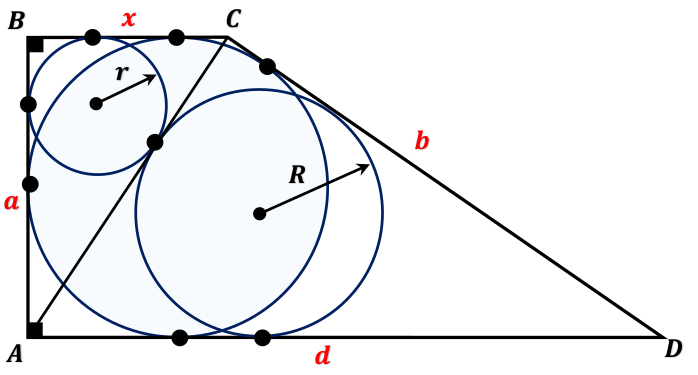
\includegraphics[width=8cm]{images/problem-1}
\end{figure}

Usando el teorema de Pitot, tenemos que $x + d = a + b$.

Al usar el teorema de Poncelet en los triángulos \theTriangle{ABC} y \theTriangle{ACD}, tenoemos que
\begin{align*}
    &a + x = AC +  2 \cdot 5 \quad \text{y} \quad AC + b = d + 2\cdot 8\\[3mm]
    &\Rightarrow (a + b) + x + AC = AC + d + 26\\
    &\Rightarrow x + d + x = d + 26\\
    &\Rightarrow 2x = 26\\
    &\Rightarrow \boxed{x = 13}.
\end{align*}

\textbf{Criterios de evaluación.}
\begin{itemize}
    \item \textbf{2 puntos.} Por realizar correctamente la gráfica (saber representar un trapecio rectángulo circunscrito, inradios, perpendicularidad y puntos de tangencias).
    \item \textbf{1 punto.} Por utilizar correctamente el teorema de Pitot $x + d = a + b$.
    \item \textbf{2 puntos.} Por usar correctamente el teorema de Poncelet (uno por cada ecuación) $a + x = AC + 10$, $AC + b = d + 16$.
    \item \textbf{2 puntos.} Por resolver y concluir que $x = 13$.
\end{itemize}



\newpage
\textbf{Problema 2.}

Escribimos la ecuación en la forma $(x^3 + 1)^2 + (x^3 + 1) = y^4 + 1$, la cual es equivalente a $(2x^3 + 3)^2 - 4y^4 = 5$.
De donde obtenemos los siguientes casos
\begin{align*}
    \begin{cases}
        2x^3 - 2y^2 + 3 = 1\\
        2x^3 + 2y^2 + 3 = 5
    \end{cases}
    &&
    \begin{cases}
        2x^3 - 2y^2 + 3 = -1\\
        2x^3 + 2y^2 + 3 = -5
    \end{cases}\\[2mm]
    \begin{cases}
        2x^3 - 2y^2 + 3 = 5\\
        2x^3 + 2y^2 + 3 = 1
    \end{cases}
    &&
    \begin{cases}
        2x^3 - 2y^2 + 3 = -5\\
        2x^3 + 2y^2 + 3 = -1
    \end{cases}
\end{align*}
Después de resolver estos sistemas, otenemos como únicas soluciones a $(0, -1)$ y $(0, -1)$.

\textbf{Criterios de evaluación.}
\begin{itemize}
    \item \textbf{3 puntos.} Por notar que la ecuación se puede expresar de la forma $(2x^3 + 3)^2 - 4y^4 = 5$.
    \item \textbf{3 puntos.} Por resolver correctamente los sistema de ecuaciones.
    \item \textbf{1 punto.} Por indicar las soluciones correctas.
\end{itemize}


\newpage
\textbf{Problema 3.}
\begin{figure}[H]
    \centering
    \begin{tikzpicture}[xscale = 1.5, yscale = 1.5]

\end{tikzpicture}
\end{figure}

Por el teorema de Ceva aplicado al triángulo \theTriangle{ABC} con los puntos $M$, $H$ y $N$ sabemos que
\[
    \ratioCM{A}{B}{C}{N}{M}{H} = 1.
\]
Como $M$ es punto medio de $BC$, entonces $BM = MC$, sustituyendo este resultado y despejando el segmento $AN$ llegamos a que
\[
    AN = NB \cdot \frac{AH}{HC} \quad \Rightarrow \quad  AN = 16 \cdot \frac{AH}{HC}
\]
Por lo tanto, solo nos basta hallar la razon $\dfrac{AH}{HC}$, para ello apliquemos el teorema de Menelao al triángulo \theTriangle{BCH} con la transversal $A - P - M$.
\[
    \ratioCM{B}{C}{H}{M}{A}{P} = 1.
\]
Ya sabemos que $BM = MC$ y por dato también sabemos que $BP = 3 PH$, al sustituir estos resultados y despejar llegamos a
\[
    \frac{CA}{AH} \cdot \frac{HP}{3HP} = 1 \quad \Rightarrow \quad  \frac{CH + HA}{AH} = 3  \quad \Rightarrow \quad  \frac{CH}{AH} + 1 = 3 \quad \Rightarrow \quad \frac{AH}{HC} = \inverseOf{2}
\]
Luego, $AN = \dfrac{16}{2} = 8$.


\textbf{Criterios de evaluación.}
\begin{itemize}
    \item \textbf{1 punto.} Por aplicar correctamente el teorema de Ceva y el teorema de Menelao.
    \item \textbf{2 puntos.} Por deducir que $AN = 16 \cdot \dfrac{AH}{HC}$.
    \item \textbf{3 puntos.} Por deducir que $\dfrac{AH}{HC} = \dfrac{1}{2}$.
    \item \textbf{1 punto.} Por indicar el valor de $AN = 8$.
\end{itemize}